% CONGRUENCE \& SEQUENCES OF TRANSFORMATIONS - WORKSHEET 0 (IN-CLASS INSTRUCTION)
\documentclass[12pt, letterpaper, fleqn]{article}

% ----------------------------------------------------------
% PACKAGES
% ----------------------------------------------------------
\usepackage{graphicx}
\usepackage{xcolor}
\usepackage[most]{tcolorbox}
\usepackage{amsmath, amssymb}
\usepackage{fancyhdr}
\usepackage[utf8]{inputenc}
\usepackage[T1]{fontenc}
\usepackage{enumitem}
\usepackage{geometry}
\usepackage{tikz}
\usepackage{needspace}
\usepackage{multicol}

\usetikzlibrary{arrows.meta, calc}

% ----------------------------------------------------------
% PAGE SETUP
% ----------------------------------------------------------
\usepackage{times}
\geometry{letterpaper, top=1.25in, bottom=1.25in, marginpar=0.5in}

% ----------------------------------------------------------
% HEADER / FOOTER
% ----------------------------------------------------------
\newcommand{\logowidth}{3cm}
\setlength{\headheight}{20pt}
\setlength{\footskip}{40pt}

\pagestyle{fancy}
\fancyhf{}
\fancyhead[C]{\small\bfseries Congruence \& Sequences of Transformations}
\fancyfoot[L]{\raisebox{2pt}{
\includegraphics[width=\logowidth]{../kss.png}}}
\fancyfoot[C]{\thepage}
\fancyfoot[R]{8.2.0}

\renewcommand{\footrulewidth}{0.2pt}

% ----------------------------------------------------------
% THEME COLOR
% ----------------------------------------------------------
\definecolor{customteal}{HTML}{2fbdb9}

% ----------------------------------------------------------
% HELPER MACROS
% ----------------------------------------------------------
\newcommand{\blank}{\underline{\hspace{2.2cm}}}
\newcommand{\blanklong}{\underline{\hspace{6.5cm}}}
\newcommand{\blankshorter}{\underline{\hspace{1.5cm}}}

% ----------------------------------------------------------
% DOCUMENT
% ----------------------------------------------------------
\begin{document}

\textbf{Name:} \underline{\hspace{5cm}}
\hfill
\textbf{Date:} \underline{\hspace{3cm}}\\

% ==========================================================
% SECTION 1: FOUNDATION
% ==========================================================
\begin{tcolorbox}[colback=customteal!20]
    \large\textcolor{black}{\textbf{Foundation: Congruence \& Sequences of Transformations}}
\end{tcolorbox}

\vspace{3mm}

\noindent
Often, a single transformation is not enough to move a figure to its target location. We can chain multiple rigid motions together, which is called a \textbf{sequence of transformations}.

\begin{itemize}
    \item \textbf{Congruence:} Two figures are defined as \textbf{congruent} if you can map one exactly onto the other using a sequence of rigid motions (translations, reflections, rotations). Because rigid motions preserve size and shape, any sequence of them will also preserve size and shape.
    \item \textbf{Order Matters:} The order in which you perform the transformations is critical. Translating and then reflecting often results in a different final image than reflecting and then translating!
\end{itemize}

\vspace{4mm}

% ==========================================================
% VISUAL REPRESENTATION
% ==========================================================
\begin{tcolorbox}[colback=white, colframe=black!25, boxrule=0.6pt, arc=4mm, left=6mm, right=6mm, top=5mm, bottom=5mm]

\textbf{Visual Representation: A Sequence of Transformations}

\medskip

\begin{center}
\begin{tikzpicture}[scale=0.7]
% Grid
\draw[step=1cm,gray!30,very thin] (-5,-5) grid (5,5);
\draw[thick,->] (-5.5,0) -- (5.5,0) node[right] {$x$};
\draw[thick,->] (0,-5.5) -- (0,5.5) node[above] {$y$};

% Original Triangle A
\filldraw[fill=blue!30, draw=blue, thick] (1,1) -- (3,1) -- (1,4) -- cycle;
\node[blue] at (1.5, 2.5) {Start ($A$)};

% Step 1: Translate down 4
\filldraw[fill=green!30, draw=green!70!black, thick] (1,-3) -- (3,-3) -- (1,0) -- cycle;
\node[green!70!black] at (2, -1.5) {Step 1 ($A'$)};
\draw[->, thick, dashed, green!70!black] (2, 1) -- (2, -2.5) node[midway, right] {Translate};

% Step 2: Reflect across y-axis
\filldraw[fill=red!30, draw=red, thick] (-1,-3) -- (-3,-3) -- (-1,0) -- cycle;
\node[red] at (-2, -1.5) {Final ($A''$)};
\draw[->, thick, dashed, red] (1, -1.5) arc (0:180:1) node[midway, above] {Reflect};

\end{tikzpicture}
\end{center}

\end{tcolorbox}

\vspace{4mm}

\newpage

% ==========================================================
% WORKED EXAMPLES
% ==========================================================
\begin{tcolorbox}[colback=customteal!20]
\large\textcolor{black}{\textbf{Applying Sequences of Transformations}}
\end{tcolorbox}

\noindent
Let's see how coordinates change with multiple steps.

\vspace{3mm}

\begin{tcolorbox}[colback=white, colframe=black!25, boxrule=0.6pt, arc=4mm, left=6mm, right=6mm, top=5mm, bottom=5mm]

\textbf{Worked Example 1: Finding Final Coordinates}

\medskip

\textbf{Problem:} Point $P(2, 3)$ is reflected across the $x$-axis, and then translated by the rule $(x-1, y+4)$. Find the final coordinates $P''$.

\medskip

\textbf{Solution:}
\begin{itemize}
    \item \textbf{Step 1 (Reflection):} Reflect across the $x$-axis means $(x, y) \rightarrow (x, -y)$. 
    \item $P' = (2, -3)$.
    \item \textbf{Step 2 (Translation):} Subtract 1 from $x$ and add 4 to $y$.
    \item $P'' = (2 - 1, -3 + 4) = (1, 1)$.
\end{itemize}

\end{tcolorbox}

\vspace{4mm}

% ==========================================================
% PRACTICE 1
% ==========================================================
\begin{tcolorbox}[colback=white!15, colframe=black, boxrule=1.5pt, arc=4mm, left=6mm, right=6mm, top=5mm, bottom=5mm]

\textbf{Guided Practice: Applying Sequences}

\medskip

\noindent
\textbf{1.} Point $B(4, 5)$ is translated left 2 units, then reflected across the $y$-axis. Find $B''$. 
\vspace{1.5cm}

\noindent
\textbf{2.} Point $M(-3, 7)$ is reflected across the $y$-axis, then translated down 2 units. 
\vspace{1.5cm}

\noindent
\textbf{3.} If Figure X can be mapped onto Figure Y using a rotation and a translation, what can we confidently say about the area of Figure X compared to Figure Y? 
\vspace{1.5cm}

\end{tcolorbox}

\newpage

% ==========================================================
% THINKING PROBLEM
% ==========================================================
\begin{tcolorbox}[colback=customteal!20]
\large\textcolor{black}{\textbf{Deeper Thinking: Reversing and Designing Sequences}}
\end{tcolorbox}

\vspace{3mm}

\begin{tcolorbox}[colback=white!15, colframe=black, boxrule=1.5pt, arc=4mm, left=6mm, right=6mm, top=5mm, bottom=5mm]

\textbf{Deeper Thinking Problem 1: Designing a Sequence}

\medskip

\noindent
You want to map the segment from $A(1, 1)$ to $B(1, 4)$ onto the segment from $A'(-1, -1)$ to $B'(-1, -4)$.

\vspace{5mm}

\noindent
\textbf{a)} Can this be done with a single translation? Explain why or why not.

\vspace{3cm}

\noindent
\textbf{b)} Describe a sequence of two rigid motions that successfully maps $AB$ onto $A'B'$.

\vspace{3cm}

\end{tcolorbox}

\vspace{4mm}

\begin{tcolorbox}[colback=white!15, colframe=black, boxrule=1.5pt, arc=4mm, left=6mm, right=6mm, top=5mm, bottom=5mm]

\textbf{Deeper Thinking Problem 2: Order Matters}

\medskip

\noindent
A dancer starts at the coordinate $(4, 4)$. They must perform two moves:
\begin{itemize}
    \item \textbf{Move 1:} Reflect across the $y$-axis.
    \item \textbf{Move 2:} Translate right 4 units.
\end{itemize}

\vspace{5mm}

\noindent
\textbf{a)} If the dancer performs Move 1 followed by Move 2, what is their final coordinate? Show your work.

\vspace{3cm}

\noindent
\textbf{b)} If the dancer accidentally performs Move 2 followed by Move 1, what is their final coordinate? Does the order matter?

\vspace{3cm}

\end{tcolorbox}

\end{document}
\end{document}
